Having established the reduction to orientations,
and the symmetry-breaking assumption of canonicity,
we now turn to the construction of a CNF formula $\phi_n$
whose unsatisfiability would imply
that every set of $n$ points
contains a $6$-hole.\footnote{
  Satisfiability of $\phi_n$ would \emph{not} necessarily imply
  the existence of a point set without a $6$-hole.
  First, the mapping from sets of points to assignments of triple orientations is not surjective.
  Second, even if it were, $\phi_n$ is tailored to looking for an unsatisfiability proof,
  using implication rather than bi-implication in some of the variable-defining clauses.
}
The formula is detailed in~\Cref{fig:full-encoding}.

\begin{figure}
  \label{fig:full-encoding}
% \begin{framed}
  \begin{spreadlines}{16pt}
\begin{gather}
\hfsetfillcolor{green!10}
\hfsetbordercolor{green!60!black}
\tikzmarkin{b}(12.0,-0.9)(-0.5,0.5)
  \cvar_{i; a,b, c} \rightarrow \left(\left(\orvar_{a,b,c} \leftrightarrow \orvar_{a, i, c}  \right) \land \left(\orvar_{a,b,c} \leftrightarrow \ov{\orvar_{a, i, b}}  \right)\right) \text{ for all } 2 \leq a < i < b < c \leq n\label{eq:insideClauses1}\\
  \cvar_{i; a,b, c} \rightarrow \left(\left(\orvar_{a,b,c} \leftrightarrow \orvar_{a, i, c}  \right) \land \left(\orvar_{a,b,c} \leftrightarrow \ov{\orvar_{b, i, c}}  \right)\right) \text{ for all } 2 \leq a < b < i < c \leq n\label{eq:insideClauses2}\\
  \tikzmarkend{b}\Big(\bigwedge_{\substack{a < i < c\\ i \neq b}} \ov{\cvar_{i; a,b,c}}\Big) \rightarrow \hvar_{a, b, c} \quad \text{ for all } 2 \leq a < b < c \leq n\label{eq:holeDefClauses1}\\
%
\tikzmarkin{a}(12.0,-0.3)(-0.5,0.5)
  \orvar_{a, b, c} \land \orvar_{a, c, d} \rightarrow \orvar_{a, b, d} \quad \text{ for all } 2 \leq a < b < c < d \leq n\label{eq:signotopeClauses11}\\
  \tikzmarkend{a}\ov{\orvar_{a, b, c}} \land \ov{\orvar_{a, c, d}} \rightarrow \ov{\orvar_{a, b, d}} \quad \text{ for all } 2 \leq a < b < c < d \leq n \label{eq:signotopeClauses12}\\
%
\hfsetfillcolor{blue!10}
\hfsetbordercolor{blue!60!black}
\tikzmarkin{c}(12.0,-0.4)(-0.5,0.6)
  % \orvar_{1, b, c} \quad \text{ for all } 2 \leq b < c \leq n \label{eq:revLexClauses}\\
  \tikzmarkend{c}\left(\orvar_{\lceil \frac{n}{2} \rceil -1, \lceil \frac{n}{2} \rceil,\lceil \frac{n}{2} \rceil+1}, \ldots, \orvar_{2,3,4} \right) \succeq_{\text{lex}} \left(\orvar_{\lfloor \frac{n}{2}\rfloor +1,  \lfloor \frac{n}{2}\rfloor +2, \lfloor \frac{n}{2}\rfloor +3}, \ldots, \orvar_{n-2, n-1, n} \right)\label{eq:revLexClauses}\\
%
\hfsetfillcolor{orange!10}
\hfsetbordercolor{orange!60!black}
\tikzmarkin{d}(12.0,-0.3)(-0.5,0.5)
  \ov{\orvar_{a,b,c}} \land \ov{\orvar_{b,c,d}} \rightarrow \uvar_{a, c, d} \quad \text{ for all } 2 \leq a < b < c < d \leq n\label{eq:capDef}\\
  \orvar_{a, b, c} \land \orvar_{b, c, d} \rightarrow \vvar_{a, c, d} \quad \text{ for all } 2 \leq a < b < c < d \leq n \label{eq:cupDef}\\
  \uvar_{a,b,c} \land \ov{\orvar_{b,c,d}} \land \hvar_{a,b,d} \rightarrow \ufvar_{a, c, d} \quad \text{ for all } 2 \leq a < b < c < d \leq n,\; a+1<b\label{eq:capFDef}\\
  \uvar_{a, c, d} \rightarrow \ov{\orvar_{a,c,d}} \quad \text{ for all } 2 \leq a < c < d \leq n,\ a+1<c\label{eq:capDef2}\\
  \tikzmarkend{d}\vvar_{a, c, d} \rightarrow \orvar_{a,c,d} \quad \text{ for all } 2 \leq a < c < d \leq n,\; a+1<c\label{eq:cupDef2}\\
%
\hfsetfillcolor{red!10}
\hfsetbordercolor{red!60!black}
\tikzmarkin{e}(12.0,-0.5)(-0.5,0.5)
  \neg(\ufvar_{a,d,e} \land \orvar_{a, p, e}) \quad \text { for all } 2 \leq a < d < e \leq n, \; a < p < e, \; a+2 < d\label{eq:no6Hole1Below}\\
  \neg(\ufvar_{a,d,e} \land \ov{\orvar_{d, e, f}}) \quad \text { for all } 2 \leq a < d < e < f\leq n, \; a+2 < d\label{eq:no6Hole4Above}\\
  \neg(\uvar_{a,c,d} \land \vvar_{a, c', d} \land \hvar_{a,c,c'}) \quad \text{ for all } 2 \leq a < c < c' < d \leq n, \; a+1 < c\label{eq:no6Hole2Below1}\\
  \neg(\uvar_{a,c,d} \land \vvar_{a, c', d} \land \hvar_{a,c',c}) \quad \text{ for all } 2 \leq a < c' < c < d \leq n, \; a+1 < c'\label{eq:no6Hole2Below2}\\
  \tikzmarkend{e}\neg(\vvar_{a,c,d} \land \orvar_{c, d, e} \land \hvar_{a,c,e}) \quad \text{ for all } 2 \leq a < c < d < e \leq n, \; a+1 < c\label{eq:no6Hole3Below}
  \end{gather}
\end{spreadlines}
% \end{framed}
\caption{Encoding based on that of Heule and Scheucher for the Empty Hexagon Number~\cite{emptyHexagonNumber}. Each line determines a set of clauses. Unsatisfiability of the formula below for $n=30$ implies $h(6) \leq 30$, as detailed throughout the paper.}
\end{figure}


\subparagraph*{Variables.}
Let $S = (p_1, \ldots, p_n)$ be the list of points in canonical position.
We explain the variables of $\phi_n$
by specifying their values in the propositional assignment $\tau_S$
that is our intended model of $\phi_n$
corresponding to $S$. We then have:
\begin{itemize}
  \item
    For every $2 \leq a < b < c \leq n$, $\orvar_{a,b,c}$ is true
    iff $\sigma(p_a,p_b,p_c) = +1$.\footnote{
    Since the point set is in general position,
    we have $\neg \orvar_{a,b,c} \iff \sigma(p_a, p_b, p_c) = -1$.}

    The first optimization observes that orientations are antisymmetric:
    if $(p,q,r)$ is counterclockwise then $(q,p,r)$ is clockwise, etc.
    Thus one only needs $\orvar_{a,b,c}$ for ordered triples $(a,b,c)$,
    reducing the number of orientation variables by a factor of $3! = 6$
    relative to using all triples. The second optimization uses the \textbf{CCW-order} property of canonical positions:
    since all $\orvar_{1,a,b}$ are true, we may as well omit them from the encoding.

  \item
    Next, for every $a < b < c$ with $a < i < b$ or $b < i < c$,
    the variable $\cvar_{i;a,b,c}$ is true
    iff \lstinline|σPtInTriangle S[i] S[a] S[b] S[c]| holds.
    By \lstinline|σPtInTriangle_iff|, this is true exactly
    iff $p_i$ is inside the triangle $p_ap_bp_c$.
    The reason for assuming $(a,b,c)$ to be ordered is again symmetry:
    $p_ap_bp_c$ is the same triangle as $p_ap_cp_b$, etc.
    Furthermore thanks to the \textbf{$x$-order} property of canonical positions,
    if $p_i$ is in the triangle
    then $x(p_a) < x(p_i) < x(p_c)$.
    This implies that $a < i < c$,
    leaving one case distinction permuting $(i,b)$.

  \item
    For every $a < b < c$,
    $\hvar_{a,b,c}$ is true
    iff \lstinline|σIsEmptyTriangleFor S[a] S[b] S[c] S| holds. 
    %  Analogously to the previous items,
    By a geometro-combinatorial connection analogous to ones above,
    this is true iff $p_ap_bp_c$ is a $3$-hole.

  \item
    Finally, one defines \emph{$4$-cap}, \emph{$5$-cap}, and \emph{$4$-cup} variables.
    For $a+1 < c < d$, $\uvar_{a,c,d}$ is true
    iff there is $b$ with $a < b < c$ with $\sigma(p_a,p_b,p_c) = \sigma(p_b,p_c,p_d) = -1$.
    $\vvar_{a,c,d}$ is analogous, except in that the two orientations are required to be counterclockwise.
    These are the $4$-caps and $4$-cups, respectively.
    The $5$-cap variables $\ufvar_{a,d,e}$
    are defined for $a+2 < d < e$.
    We set $\ufvar_{a,d,e}$ to true
    iff there exists $c$ with $a+1<c<d$
    such that $\uvar_{a,c,d}$, $\orvar_{c,d,e}$, and $\hvar_{a,c,e}$ are all true.
    Intuitively, $4$-caps and $4$-cups are clockwise and counterclockwise arcs of length $4$,
    respectively,
    whereas $5$-caps are clockwise arcs of length $5$ containing a $3$-hole.
    All three are depicted in~\Cref{fig:cup-cap-vars}. The usage of these variables is crucial to an efficient encoding:
    we will show below that a hexagon can be covered by only $4$ triangles,
    so one need not consider all ${6\choose 3}$ triangles contained within it.
\end{itemize}

\begin{figure}
\centering
\begin{subfigure}{0.3\textwidth}
    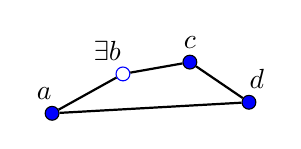
\begin{tikzpicture}
        \node[draw, circle, black, fill=blue, inner sep=0pt, minimum size=5pt,label={[xshift=-0.1cm, yshift=-0.05cm]$a$}] (a) at (0,0) {};
        \node[draw, circle, blue,  inner sep=0pt, minimum size=5pt, label={[xshift=-0.2cm, yshift=-0.05cm]$\exists b$}] (b) at (0.9*1,1*0.5) {};
        \node[draw, circle, black, fill=blue, inner sep=0pt, minimum size=5pt, label={[xshift=-0.0cm, yshift=-0.05cm]$c$}] (c) at (1.75*1, 1.3*0.5) {};
        \node[draw, circle, black, fill=blue, inner sep=0pt, minimum size=5pt, label={[xshift=0.1cm, yshift=-0.05cm]$d$}] (d) at (2.5*1,0.2*0.7) {};
    \draw[thick] (a) -- (b) -- (c) -- (d) -- (a);
    \end{tikzpicture}
    \caption{$\uvar_{a,c,d}$}\label{fig:cap}
\end{subfigure}
\begin{subfigure}{0.3\textwidth}
    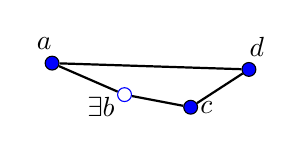
\begin{tikzpicture}
        \node[draw, circle, black, fill=blue, inner sep=0pt, minimum size=5pt,label={[xshift=-0.1cm, yshift=-0.05cm]$a$}] (a) at (0,0) {};
        \node[draw, circle, blue,  inner sep=0pt, minimum size=5pt, label={[xshift=-0.3cm, yshift=-0.5cm]$\exists b$}] (b) at (0.92*1,-0.5*0.8) {};
        \node[draw, circle, black, fill=blue, inner sep=0pt, minimum size=5pt, label={[xshift=0.2cm, yshift=-0.3cm]$c$}] (c) at (1.6*1.1, -0.7*0.8) {};
        \node[draw, circle, black, fill=blue, inner sep=0pt, minimum size=5pt, label={[xshift=0.1cm, yshift=-0.05cm]$d$}] (d) at (2.5*1,-0.2*0.4) {};
    \draw[thick] (a) -- (b) -- (c) -- (d) -- (a);
    \end{tikzpicture}
    \caption{$\vvar_{a,c,d}$}\label{fig:cup}
\end{subfigure}
\begin{subfigure}{0.35\textwidth}
    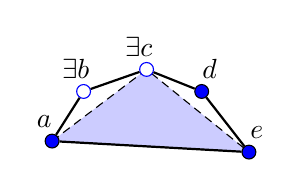
\begin{tikzpicture}
  
    \coordinate (a) at (0,0);
    \coordinate (c) at (1.2*1, 1.3*0.7);
    \coordinate (e) at (2.5*1,-0.2*0.7);
    \fill[blue, opacity=0.2] (a) -- (c) -- (e) -- cycle;
    \draw[densely dashed] (a) -- (c) -- (e) -- (a);

    \node[draw, circle, black, fill=blue, inner sep=0pt, minimum size=5pt,label={[xshift=-0.1cm, yshift=-0.05cm]$a$}] (a) at (0,0) {};
    \node[draw, circle, blue,  fill=white, inner sep=0pt, minimum size=5pt, label={[xshift=-0.1cm, yshift=-0.05cm]$\exists b$}] (b) at (0.4*1,0.9*0.7) {};
    \node[draw, circle, blue, fill=white, inner sep=0pt, minimum size=5pt, label={[xshift=-0.1cm, yshift=-0.05cm]$\exists c$}] (c) at (1.2*1, 1.3*0.7) {};
    \node[draw, circle, black, fill=blue, inner sep=0pt, minimum size=5pt, label={[xshift=0.1cm, yshift=-0.05cm]$d$}] (d) at (1.9*1,0.9*0.7) {};
    \node[draw, circle, black, fill=blue, inner sep=0pt, minimum size=5pt, label={[xshift=0.1cm, yshift=-0.05cm]$e$}] (e) at (2.5*1,-0.2*0.7) {};

    \draw[thick] (a) -- (b) -- (c) -- (d) -- (e) -- (a);
    \end{tikzpicture}
    \caption{$\ufvar_{a,d,e}$}\label{fig:5cap}
\end{subfigure}

\caption{Illustration of the $4$-caps (\ref{fig:cap}), $4$-cups (\ref{fig:cup}), and $5$-caps (\ref{fig:5cap}) variables.  The highlighted region denotes an empty triangle.}\label{fig:cup-cap-vars}
\end{figure}

\begin{figure}
    \centering
    \begin{subfigure}{0.3\textwidth}
        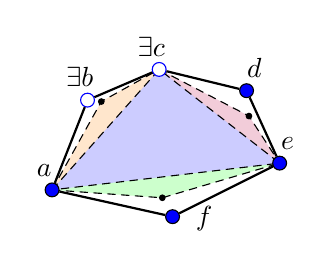
\begin{tikzpicture}
        
    
    
        \coordinate (a) at (0,0);
        \coordinate (c) at (0.8*1.7, 0.9*1.7);
        \coordinate (e) at (1.7*1.7,0.2*1.7);

        \coordinate (p1) at (0.25*2.5, 0.66*1.7);
        \coordinate (p2) at (2.5,0.67*1.4);
        \coordinate (p3) at (1.4,-0.1);

        \fill[blue, opacity=0.2] (a) -- (c) -- (e) -- cycle;
        \fill[orange, opacity=0.2] (a) -- (p1) -- (c) -- cycle;
        \fill[purple, opacity=0.2] (c) -- (p2) -- (e) -- cycle;
        \fill[green, opacity=0.2] (a) -- (p3) -- (e) -- cycle;
        \draw[densely dashed] (a) -- (c) -- (e) -- (a);

        \draw[densely dashed] (a) -- (p1) -- (c);
        \draw[densely dashed] (a) -- (p3) -- (e);
        \draw[densely dashed] (c) -- (p2) -- (e);

        \node[draw, circle, black, fill=blue, inner sep=0pt, minimum size=5pt,label={[xshift=-0.1cm, yshift=-0.05cm]$a$}] (a) at (0,0) {};
        \node[draw, circle, blue, fill=white, inner sep=0pt, minimum size=5pt, label={[xshift=-0.1cm, yshift=-0.05cm]$\exists b$}] (b) at (0.3*1.5,0.6*1.9) {};
        \node[draw, circle, blue, fill=white, inner sep=0pt, minimum size=5pt, label={[xshift=-0.1cm, yshift=-0.05cm]$\exists c$}] (c) at (0.8*1.7, 0.9*1.7) {};
        \node[draw, circle, black, fill=blue, inner sep=0pt, minimum size=5pt, label={[xshift=0.1cm, yshift=-0.05cm]$d$}] (d) at (1.3*1.9,0.7*1.8) {};
        \node[draw, circle, black, fill=blue, inner sep=0pt, minimum size=5pt, label={[xshift=0.1cm, yshift=-0.05cm]$e$}] (e) at (1.7*1.7,0.2*1.7) {};
        \node[draw, circle, black, fill=blue, inner sep=0pt, minimum size=5pt, label={[xshift=0.4cm, yshift=-0.4cm]$f$}] (f) at (0.9*1.7,-0.2*1.7) {};
        \draw[thick] (a) -- (b) -- (c) -- (d) -- (e) -- (f) -- (a);
    
        \node[draw, circle, black, fill=black, inner sep=0pt, minimum size=2pt] (p1) at (0.25*2.5,0.66*1.7) {};
        \node[draw, circle, black, fill=black, inner sep=0pt, minimum size=2pt] (p2) at (2.5,0.67*1.4) {};
        \node[draw, circle, black, fill=black, inner sep=0pt, minimum size=2pt] (p3) at (1.4,-0.1) {};
        \end{tikzpicture}
        \caption{$(\ufvar_{a,d,e} \land \orvar_{a,f,e})$}\label{fig:clause-13-forbid}
    \end{subfigure}
    \begin{subfigure}{0.3\textwidth}
        \begin{tikzpicture}
      
       
        \newcommand{\scalefact}{1.3}
        \coordinate (a) at (0*\scalefact,0*\scalefact);
        \coordinate (c) at (0.8*1.7*\scalefact, 0.9*1.7*\scalefact);
        \coordinate (e) at (1.7*1.7*\scalefact,0.2*1.7*\scalefact);

       \coordinate (p1) at (0.25*2.5*\scalefact, 0.66*1.55*\scalefact);
        \coordinate (p2) at (1.8*\scalefact,0.66*1.7*\scalefact);
       \coordinate (bp) at (1.2*\scalefact,0.1*\scalefact);
         \coordinate (cp) at (1.8*\scalefact,0.67*0.8*\scalefact);

        

        \fill[blue, opacity=0.2] (a) -- (c) -- (cp) -- cycle;
        \fill[orange, opacity=0.2] (a) -- (p1) -- (c) -- cycle;
        \fill[purple, opacity=0.2] (c) -- (p2) -- (cp) -- cycle;
       
         \fill[green, opacity=0.2] (a) -- (cp) -- (bp) -- cycle;
    

        \draw[densely dashed] (a) -- (c) -- (cp) -- (a);
        \draw[densely dashed] (a) -- (p1) -- (c);
        \draw[densely dashed] (c) -- (p2) -- (cp);

        \node[draw, circle, black, fill=blue, inner sep=0pt, minimum size=5pt,label={[xshift=-0.1cm, yshift=-0.05cm]$a$}] (a) at (0*\scalefact,0*\scalefact) {};
        \node[draw, circle, blue,  fill=white, inner sep=0pt, minimum size=5pt, label={[xshift=-0.1cm, yshift=-0.05cm]$\exists b$}] (b) at (0.3*1.5*\scalefact,0.6*1.9*\scalefact) {};
        \node[draw, circle, black, fill=blue, inner sep=0pt, minimum size=5pt, label={[xshift=-0.1cm, yshift=-0.05cm]$c$}] (c) at (0.8*1.7*\scalefact, 0.9*1.7*\scalefact) {};
        \node[draw, circle, black, fill=blue, inner sep=0pt, minimum size=5pt, label={[xshift=0.1cm, yshift=-0.05cm]$d$}] (d) at (1.1*1.9*\scalefact,0.7*1.8*\scalefact) {};
        % \node[draw, circle, black, fill=blue, inner sep=0pt, minimum size=5pt, label={[xshift=0.1cm, yshift=-0.05cm]$e$}] (e) at (1.7*1.7,0.2*1.7) {};
        % \node[draw, circle, black, fill=blue, inner sep=0pt, minimum size=5pt, label={[xshift=0.4cm, yshift=-0.4cm]$f$}] (f) at (0.9*1.7,-0.2*1.7) {};
      
    
        \node[draw, circle, black, fill=black, inner sep=0pt, minimum size=2pt] (p1) at (0.25*2.5*\scalefact,0.66*1.55*\scalefact) {};
        \node[draw, circle, black, fill=black, inner sep=0pt, minimum size=2pt] (p2) at (1.8*\scalefact,0.66*1.7*\scalefact) {};

        \node[draw, circle, black, fill=blue, inner sep=0pt, minimum size=5pt, label={[xshift=0.3cm, yshift=-0.2cm]$c'$}] (cp) at (1.8*\scalefact,0.67*0.8*\scalefact) {};
        \node[draw, circle, blue,  fill=white, inner sep=0pt, minimum size=5pt, label={[xshift=0.5cm, yshift=-0.4cm]$\exists b'$}] (bp) at (1.2*\scalefact,0.1*\scalefact) {};

        \draw[thick] (a) -- (b) -- (c) -- (d) -- (cp)  -- (bp) -- (a);
        % \draw[densely dashed] (a) -- (p3) -- (e);
        % \draw[densely dashed] (c) -- (p2) -- (e);
        \end{tikzpicture}
        \caption{$(\uvar_{a,c,d} \land \vvar_{a, c', d} \land \hvar_{a,c,c'})$}\label{fig:clause-14-forbid}
    \end{subfigure}
    \begin{subfigure}{0.3\textwidth}
        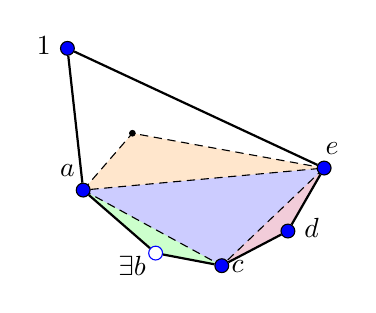
\begin{tikzpicture}
           
        % \node[draw, circle, black, fill=black, inner sep=0pt, minimum size=2pt] (p2) at (2.5,0.67*1.4) {};
        % \node[draw, circle, black, fill=black, inner sep=0pt, minimum size=2pt] (p3) at (1.4,-0.1) {};
    
    
        \coordinate (a) at (0,0.4);
        \coordinate (b) at (0.92*1,-0.5*0.8);
        \coordinate (c) at (1.6*1.1, -0.7*0.8);
        \coordinate (d) at (2.6*1,-0.3*0.4);
        \coordinate (e) at (1.8*1.7,0.4*1.7);

        \coordinate (p1) at (0.25*2.5, 0.66*1.7);
        \coordinate (p2) at (2.5,0.67*1.4);
        \coordinate (p3) at (1.4,-0.1);

        \fill[blue, opacity=0.2] (a) -- (c) -- (e) -- cycle;
         \fill[orange, opacity=0.2] (a) -- (p1) -- (e) -- cycle;
        \fill[purple, opacity=0.2] (c) -- (d) -- (e) -- cycle;
        \fill[green, opacity=0.2] (a) -- (b) -- (c) -- cycle;
        % \draw[densely dashed] (a) -- (c) -- (e) -- (a);


         \draw[densely dashed] (a) -- (c) -- (e) -- (a);

       
        \draw[densely dashed] (a) -- (p1) -- (e);

        \node[draw, circle, black, fill=blue, inner sep=0pt, minimum size=5pt,label={[xshift=-0.2cm, yshift=-0.05cm]$a$}] (a) at (0,0.4) {};
        \node[draw, circle, blue,  fill=white, inner sep=0pt, minimum size=5pt, label={[xshift=-0.3cm, yshift=-0.5cm]$\exists b$}] (b) at (0.92*1,-0.5*0.8) {};
        \node[draw, circle, black, fill=blue, inner sep=0pt, minimum size=5pt, label={[xshift=0.2cm, yshift=-0.3cm]$c$}] (c) at (1.6*1.1, -0.7*0.8) {};
        \node[draw, circle, black, fill=blue, inner sep=0pt, minimum size=5pt, label={[xshift=0.3cm, yshift=-0.3cm]$d$}] (d) at (2.6*1,-0.3*0.4) {};
        \node[draw, circle, black, fill=blue, inner sep=0pt, minimum size=5pt, label={[xshift=-0.3cm, yshift=-0.3cm]$1$}] (1) at (-0.2*1,2.2) {};
        

    % \node[draw, circle, black, fill=blue, inner sep=0pt, minimum size=5pt,label={[xshift=-0.1cm, yshift=-0.05cm]$a$}] (a) at (0,0) {};
    % \node[draw, circle, blue,  inner sep=0pt, minimum size=5pt, label={[xshift=-0.1cm, yshift=-0.05cm]$\exists b$}] (b) at (0.3*1.5,0.6*1.9) {};
    % \node[draw, circle, blue, inner sep=0pt, minimum size=5pt, label={[xshift=-0.1cm, yshift=-0.05cm]$\exists c$}] (c) at (0.8*1.7, 0.9*1.7) {};
    % \node[draw, circle, black, fill=blue, inner sep=0pt, minimum size=5pt, label={[xshift=0.1cm, yshift=-0.05cm]$d$}] (d) at (1.3*1.9,0.7*1.8) {};
    \node[draw, circle, black, fill=blue, inner sep=0pt, minimum size=5pt, label={[xshift=0.1cm, yshift=-0.05cm]$e$}] (e) at (1.8*1.7,0.4*1.7) {};
    % \node[draw, circle, black, fill=blue, inner sep=0pt, minimum size=5pt, label={[xshift=0.4cm, yshift=-0.4cm]$f$}] (f) at (0.9*1.7,-0.2*1.7) {};
    % \draw[thick] (a) -- (b) -- (c) -- (d) -- (e) -- (f) -- (a);

 \node[draw, circle, black, fill=black, inner sep=0pt, minimum size=2pt] (p1) at (0.25*2.5,0.66*1.7) {};
 \draw[thick] (1) -- (a) -- (b) -- (c) -- (d) -- (e) -- (1);
        % \draw[densely dashed] (c) -- (p2) -- (e);
        \end{tikzpicture}
        \caption{$(\vvar_{a,c,d} \land \orvar_{c, d, e} \land \hvar_{a,c,e})$}\label{fig:clause-15-forbid}
    \end{subfigure}
    \caption{Illustration of some \emph{forbidden configurations} that imply $6$-holes. \Cref{fig:clause-13-forbid} corresponds to the configuration forbidden by~\Cref{eq:no6Hole1Below}, \Cref{sub@fig:clause-14-forbid} to the one forbidden by~\Cref{eq:no6Hole2Below1}, and~\Cref{fig:clause-15-forbid} to~\Cref{eq:no6Hole3Below}. All highlighted regions correspond to empty triangles.}\label{fig:forbidden}
\end{figure}


\subparagraph*{Satisfaction.}
We now have to justify that the clauses of $\phi_n$
are satisfied by the intended interpretation $\tau_S$
for a $6$-hole-free point set $S$.
The variable-defining clauses~\labelcref{eq:insideClauses1,eq:insideClauses2,eq:holeDefClauses1,eq:capDef,eq:cupDef,eq:capFDef,eq:capDef2,eq:cupDef2}
follow essentially by definition combined with boolean reasoning.
The orientation properties~\labelcref{eq:signotopeClauses11,eq:signotopeClauses12}
have been established in the family of theorems \lstinline|σ_propᵢ|.
The lexicographic ordering clauses~\labelcref{eq:revLexClauses}
follow from the \textbf{Lex order} property of canonical positions.
Thus we are left with clauses~\labelcref{eq:no6Hole1Below,eq:no6Hole4Above,eq:no6Hole2Below1,eq:no6Hole2Below2,eq:no6Hole3Below}
which forbid the presence of certain $6$-holes.\footnote{
They are intended to forbid \emph{all} $6$-holes,
but we do not prove completeness.}
We illustrate it for clause~\labelcref{eq:no6Hole1Below}.
The contrapositive is easier to state:
if $\tau_S(\ufvar_{a,d,e}) = \tau_S(\orvar_{a,p,e}) = 1$,
then $S$ contains a $6$-hole.
The intuitive argument is depicted in~\Cref{fig:clause-13-forbid}.
We know that $aec$ forms a $3$-hole,
and wish to conclude the existence of a $6$-hole.
If $ape$, $edc$, and $cba$ are all $3$-holes,
then we are done
by gluing the four triangles into an empty hexagon.
Suppose otherwise that $ape$ were not a $3$-hole,
i.e., there is a nonempty set $O$
of points strictly contained in $ape$.
Then we can take the element $\cdot \in O$ closest to $ea$,
and construct a new triangle $\cdot ea$, in green.
By minimality of distance between $\cdot$ and $ea$,
this is a $3$-hole.
Repeating the argument for $edc$ and $cba$ concludes the proof.

Justifying this reasoning formally
turned to be complex,
requring a fair bit of reasoning about point \lstinline|Arc|s
and \lstinline|σCCWPoints|: lists of points winding around a convex polygon.
Luckily, the main argument can be summarized in terms of two facts:
(a) the minimality argument works; and
(b) empty shapes sharing a common line segment can be glued together.
Formally, (a) can be stated as

\begin{lstlisting}
theorem σIsEmptyTriangleFor_exists (gp : ListInGenPos S)
  (abc : [a, b, c] ⊆ S) :
  ∃ b' ∈ S, σ a b' c = σ a b c ∧ (b' = b ∨ σPtInTriangle b' a b c) ∧
    σIsEmptyTriangleFor a b' c S.toFinset
\end{lstlisting}
\begin{proof}
  Given points $p,q$, say that $p \leq q$ iff $p$ is in the triangle $aqc$.
  This is a preorder.
  Now, the set $S' = \{x \in S \mid \sigma(a,x,c) = \sigma(a,b,c) \wedge x \leq b\}$
  is finite and so has a weakly minimal element $b'$,
  in the sense that no $x \in S'$ has $x < b'$.
  Emptiness of $ab'c$ follows by minimality.
\end{proof}

Moving on, (b) follows from a \emph{triangulation lemma}:
given any convex point set $S$
and a line $\overleftrightarrow{ab}$ between vertices of $S$,
the convex hull of $S$ is contained in the convex hull
of points on each side of $\overleftrightarrow{ab}$.
That is:
\begin{lstlisting}
theorem split_convexHull (cvx : ConvexPoints S) :
  ∀ {a b}, a ∈ S → b ∈ S →
    convexHull ℝ S ⊆
    convexHull ℝ {x ∈ S | σ a b x ≠ ccw} ∪
    convexHull ℝ {x ∈ S | σ a b x ≠ cw}
\end{lstlisting}
\begin{figure}
    \centering
    \begin{subfigure}{0.45\textwidth}
        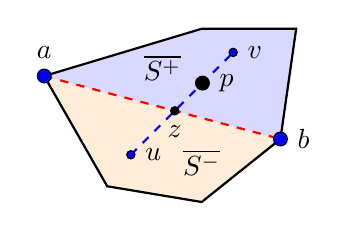
\begin{tikzpicture}
        \coordinate (a) at (0, 0.4);
        \coordinate (b) at (3, -0.4);
        \coordinate (v1) at (3.2, 1);
        \coordinate (v2) at (2, 1);
        \coordinate (u1) at (0.8, -1);
        \coordinate (u2) at (2, -1.2);
        \coordinate (u) at (1.1, -0.6);
        \coordinate (v) at (2.4, 0.7);
        \coordinate (p) at (2.01,0.31);
        \coordinate (z) at (1.65789, -0.0421053);

        \fill[blue, opacity=0.15] (b) -- (v1) -- (v2) -- (a) -- cycle;
        \fill[orange, opacity=0.15] (a) -- (u1) -- (u2) -- (b) -- cycle;

        \draw[thick] (a) -- (u1) -- (u2) -- (b) -- (v1) -- (v2) -- (a);
        \draw[dashed, thick, red] (a) -- (b);
        \draw[dashed, thick, blue] (u) -- (v);

        \node[draw, circle, black, fill=blue, inner sep=0pt, minimum size=5pt, label=above:$a$] (pA) at (a) {};
        \node[draw, circle, black, fill=blue, inner sep=0pt, minimum size=5pt, label=right:$b$] (pB) at (b) {};
        \node[draw, circle, black, fill=blue, inner sep=0pt, minimum size=3pt, label=right:$u$] (pU) at (u) {};
        \node[draw, circle, black, fill=blue, inner sep=0pt, minimum size=3pt, label=right:$v$] (pV) at (v) {};

        \node[draw, circle, black, fill=black, inner sep=0pt, minimum size=5pt, label=right:$p$] (pP) at (p) {};
        \node[draw, circle, black, fill=black, inner sep=0pt, minimum size=3pt, label=below:$z$] (pZ) at (z) {};

        \node[] at (1.5, 0.5) {$\overline{S^+}$};
        \node[] at (2, -0.7) {$\overline{S^-}$};

        \end{tikzpicture}
        \caption{}\label{fig:triangulation2-a}
    \end{subfigure}
    \begin{subfigure}{0.45\textwidth}
        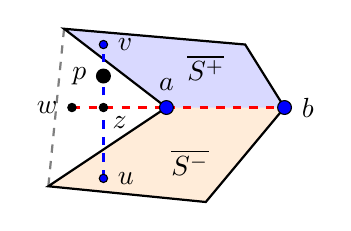
\begin{tikzpicture}
            \coordinate (a) at (1.5, 0);
            \coordinate (b) at (3, 0);
            \coordinate (v1) at (2.5, 0.8);
            \coordinate (v2) at (0.2, 1);
            \coordinate (u1) at (0, -1);
            \coordinate (u2) at (2, -1.2);
            \coordinate (u) at (0.7, -0.9);
            \coordinate (v) at (0.7, 0.8);
            \coordinate (p) at (0.7, 0.4);
            \coordinate (z) at (0.7, 0);
            \coordinate (w) at (0.3, 0);

            \fill[blue, opacity=0.15] (b) -- (v1) -- (v2) -- (a) -- cycle;
            \fill[orange, opacity=0.15] (a) -- (u1) -- (u2) -- (b) -- cycle;

            \draw[thick] (a) -- (u1) -- (u2) -- (b) -- (v1) -- (v2) -- (a);
            \draw[dashed, thick, red] (a) -- (b);
            \draw[dashed, thick, blue] (u) -- (v);
            \draw[dashed, thick, red] (w) -- (a);
            \draw[dashed, thick, opacity=0.5] (v2) -- (u1);

            \node[draw, circle, black, fill=blue, inner sep=0pt, minimum size=5pt, label=above:$a$] (pA) at (a) {};
            \node[draw, circle, black, fill=blue, inner sep=0pt, minimum size=5pt, label=right:$b$] (pB) at (b) {};
            \node[draw, circle, black, fill=blue, inner sep=0pt, minimum size=3pt, label=right:$u$] (pU) at (u) {};
            \node[draw, circle, black, fill=blue, inner sep=0pt, minimum size=3pt, label=right:$v$] (pV) at (v) {};

            \node[draw, circle, black, fill=black, inner sep=0pt, minimum size=5pt, label=left:$p$] (pP) at (p) {};
            \node[draw, circle, black, fill=black, inner sep=0pt, minimum size=3pt, label={[shift={(-0.05,0.05)}]-45:$z$}] (pZ) at (z) {};
            \node[draw, circle, black, fill=black, inner sep=0pt, minimum size=3pt, label=left:$w$] (pW) at (w) {};

            \node[] at (2, 0.5) {$\overline{S^+}$};
            \node[] at (1.8, -0.7) {$\overline{S^-}$};

        \end{tikzpicture}
        \caption{}\label{fig:triangulation2-b}
    \end{subfigure}
    \caption{Illustration of the proof for \lstinline|split_convexHull|. (a) Given point $p$, we obtain points $u$ and $v$ inside the two halves and $z$ as the point of intersection with the line $\overline{ab}$. (b) In this (contradictory) situation, the point $z$ has ended up outside the segment $\overline{ab}$, because $S$ is not actually convex. In this case we construct $w$ such that $z$ is on the $\overline{wa}$ segment, and observe that $w,z,a,b$ are collinear.}\label{fig:triangulation2}
\end{figure}

\begin{proof}
    Let $S^+=\{x\in S\mid \sigma(a,b,x)\ge 0\}$ and $S^-=\{x\in S\mid \sigma(a,b,x)\le 0\}$ be the two sets in the theorem, and let $p\in \overline{S}$, where $\overline{S}$ denotes the convex hull of $S$. Assume WLOG that $\sigma(a,b,p)\ge 0$. (We would like to show that $p\in \overline{S^+}$.) Now $p$ is a convex combination of elements of $S^+$ and elements of $S^-$, so there exist points $u\in \overline{S^-}$ and $v\in \overline{S^+}$ such that $p$ lies on the $\overline{uv}$ line.
% 
    Because $\{x\mid \det(a,b,x)\le 0\}\supseteq S^-$ is convex, it follows that $\det(a,b,u)\le 0$, and likewise $\det(a,b,v)\ge 0$, so they lie on opposite sides of the $\overleftrightarrow{ab}$ line and hence $\overline{uv}$ intersects $\overleftrightarrow{ab}$ at a point $z$. The key point is that $z$ must in fact be on the line segment $\overline{ab}$; assuming that this was the case, we could obtain $z$ as a convex combination of $a$ and $b$, and $p$ as a convex combination of $v$ and $z$, and since $v$ is in $\overline{S^+}$ and $a,b\in S^+\subseteq\overline{S^+}$ we can conclude $p\in \overline{S^+}$.
% 
    To show that $z\in \overline{ab}$, suppose not, so that $a$ lies between $z$ and $b$ (see \Cref{fig:triangulation2-b}). (The case where $z$ is on the $b$ side is similar.) We can decompose $z$ as a convex combination of some $w\in \overline{S\setminus\{a\}}$ and $a$, which means that $w,z,a,b$ are collinear and appear in this order on the line. Therefore $a$ is a convex combination of $w$ and $b$, which means that $a\in \overline{S\setminus\{a\}}$ which violates convexity of $S$.
\end{proof}

By contraposition,
the triangulation lemma directly implies that
if $\{x \in S \mid \sigma(a,b,x) \neq +1\}$ and $\{x \in S \mid \sigma(a,b,x) \neq -1\}$
are both empty shapes in $P$,
then $S$ is an empty shape in $P$.

\subparagraph*{Running the CNF.}
Having now shown that if $\phi_{30}$ were unsatisfiable,
our main result would follow,
we run a distributed computation to confirm the antecedent
and conclude the proof.
We solve the SAT formula $\phi_{30}$ produced by Lean using the same setup as 
Heule and Scheucher~\cite{emptyHexagonNumber}, although using different hardware:
the Bridges 2 cluster of the Pittsburgh Supercomputing Center. 
Following Heule and Scheucher,
we use a partition of the problem into 312\,418 subproblems.
Each of these subproblems was
solved using {\tt CaDiCaL} version 1.9.5.
The solver produced an LRAT proof for each execution,
which was validated using the {\tt cake\_lpr} verified checker on-the-fly
in order to avoid writing/storing/reading large files. 
The total runtime was 25876.5 CPU hours, or roughly 3 CPU years.
The difference in runtime relative to Heule and Scheucher's original run
is purely due to the difference in hardware.
Additionally,
we validated that the subproblems cover the entire search space. 
This was done by verifying the unsatisfiability
of another formula that took 20 seconds to solve. 

% file-local attic:

% By using the triangulation lemma repeatedly,
% we can slice up a convex $k$-gon into smaller pieces in any way we like until we get to triangles,
% thereby showing that convex polygons can be triangulated.
